\chapter{PHƯƠNG PHÁP NGHIÊN CỨU}\label{chap2_intro}
\vspace{-40pt}

 
\section{PHƯƠNG PHÁP NGHIÊN CỨU}
Nội dung đoạn 1


Nội dung đoạn 2 nếu có
%\cite{pham2024luanvan}



\section{PHÂN TÍCH - THIẾT KẾ}
\subsection{Phân tích 1}
Nội dung văn bản
%-- Nếu có hình ---
\begin{figure}[htbp]
    \centering
    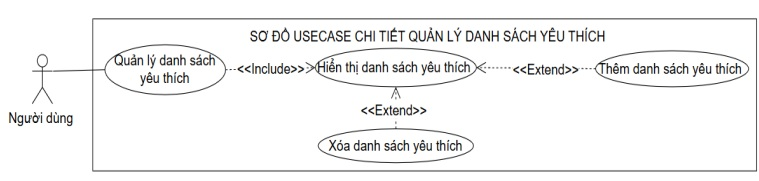
\includegraphics[width=\textwidth]{Chapter_2/Images_c2/usecase.jpg}
    \caption{Sơ đồ use case quản lý danh sách yêu thích} 
    \label{fig-usqlds}
\end{figure}

%-- Nếu có bảng ---
\begin{table}[H]
\centering
\caption{Kết quả thực nghiệm.}
\begin{tabular}{ccccc}
\toprule
\textbf{STT} & \textbf{Model}   & \textbf{Cột A} & \textbf{Cột B} & \textbf{Cột C} \\ 
\midrule
1 & Thuật toán 1        & 1  & 2  & 3            \\
2 & Thuật toán 2       & 4  & 5  & 6            \\
\bottomrule
\end{tabular}
\label{tab-kq}
\end{table}

\subsection{Phân tích 2}

\subsection{Phân tích 3}

\section{KHẢO SÁT - XỬ LÝ SỐ LIỆU MÔ HÌNH, QUY TRÌNH, CÔNG CỤ SỬ DỤNG}

\subsection{KHẢO SÁT - XỬ LÝ SỐ LIỆU MÔ HÌNH}
\subsection{QUY TRÌNH}
\subsection{CÔNG CỤ SỬ DỤNG}
